\begin{figure}[p]
    \centering
    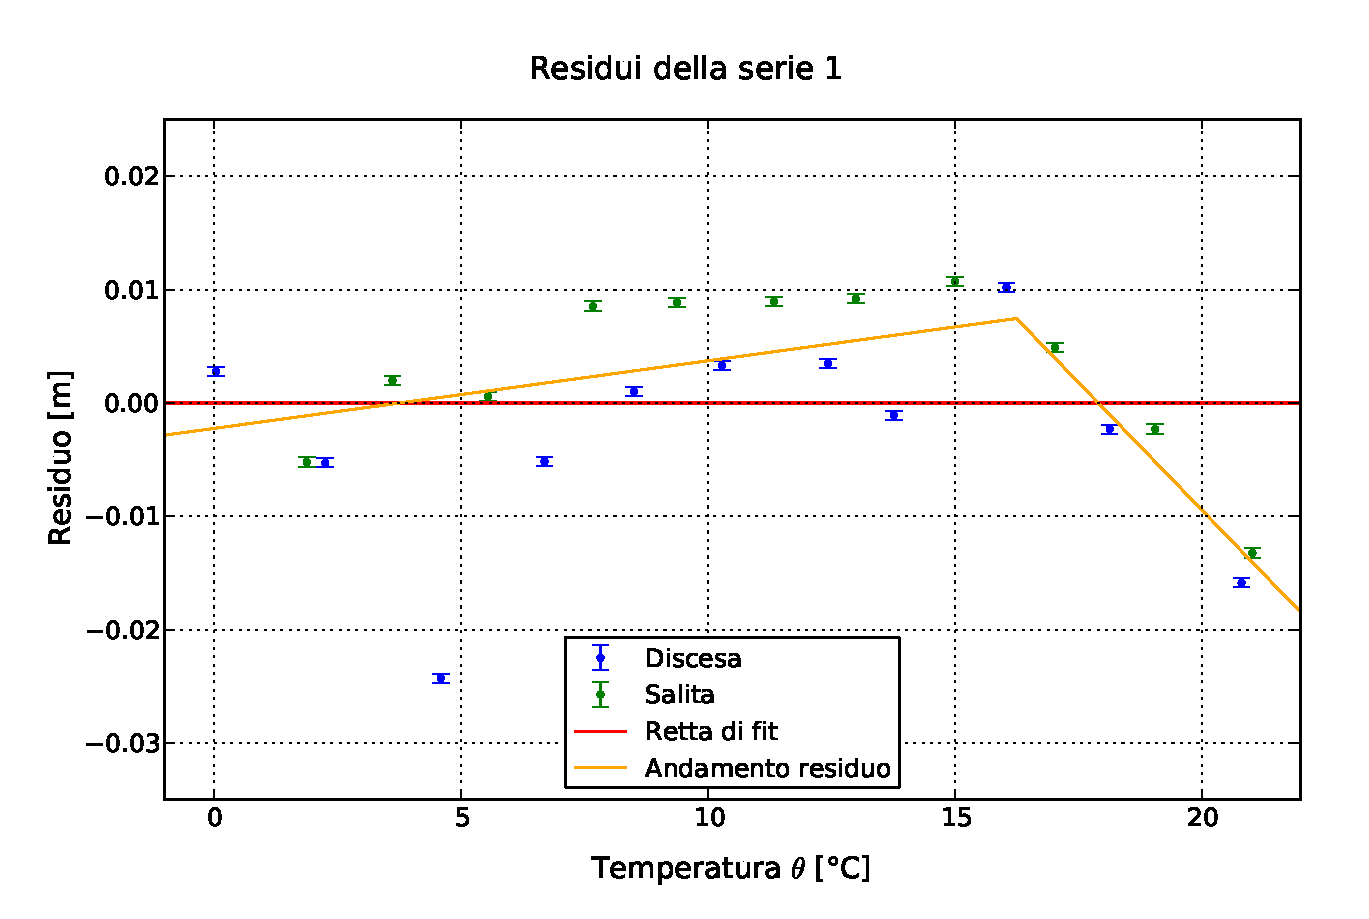
\includegraphics[width=130mm]{immagini/fit1.pdf}
    \caption{Il grafico in figura mostra i residui del fit sulla prima serie di dati. Sono riportati in colori
    diversi i dati presi abbassando (discesa) la temperatura e alzandola (salita). È evidente un andamento residuo nei dati,
    indicato approssimativamente in figura, probabilmente dovuto alla condensazione del vapor acqueo nella bottiglia. L'andamento
    residuo è formato da due rette che si incontrano attorno ai \SI{15}{\celsius}. L'ipotesi è che l'andamento residuo sia dovuto alla
    formazione di condensa all'interno del vaso, che rimuovendo molecole di gas dal recipiente, ha fatto abbassare la pressione e modificato
    la proporzionalità tra dislivello (pressione) e temperatura. C'è anche
    un dato con un residuo molto alto, visibile a sinistra della legenda.}
    \label{fig:fit1}
\end{figure}

\begin{figure}[p]
    \centering
    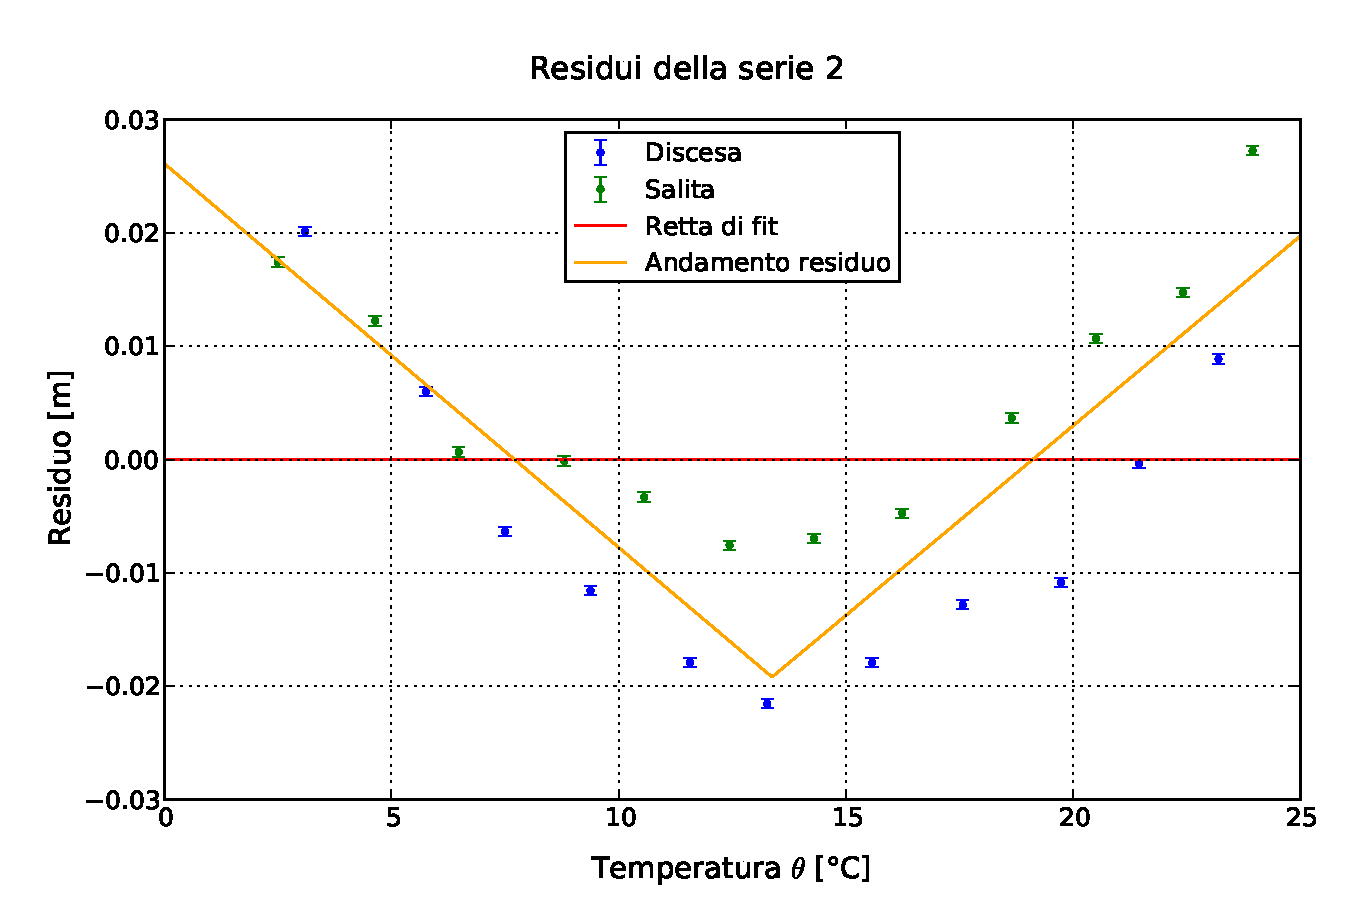
\includegraphics[width=130mm]{immagini/fit2.pdf}
    \caption{}
    \label{fig:fit2}
\end{figure}

\subsubsection{Regressione residui}

Nei paragrafi precedenti si sono riscontrati degli evidenti andamenti residui. Come conseguenza la legge lineare ottenuta
si adatta male ai dati, il $\chi^2$ è molto alto, come alte sono le correzioni da apportare alle incertezze affinché 
il valore del chi quadro risulti corretto. Certo, l'incertezza stimata inizialmente, che tiene conto solo degli errori di risoluzione
è sicuramente sottostimata e va corretta, ma portare l'incertezza sulla temperatura sino a \SI{0.3}{\celsius} non è accettabile.
Inoltre gli andamenti residui indicano che ci sono stati dei processi di cui non si è tenuto conto durante l'esecuzione dell'esperimento.

Poiché gli andamenti residui sono ben rappresentati da rette spezzate, abbiamo pensato di ovviare a tutti questi problemi suddividendo i
dati in vari gruppi in base agli andamenti residui, in modo da poter eseguire la regressione lineare per ogni gruppo di dati.
Abbiamo fatto quanto segue:

\label{sottoserie}
\begin{itemize}
    \item{Innanzitutto abbiamo eliminato un dato nella prima serie di misure, in quanto era probabilmente il frutto di un
        errore di misura. Questo dato, visibile in figura \ref{fig:fit1} a fianco della legenda,
        contribuiva molto al valore del $\chi^2$, ed era completamente scollegato dal resto della serie.}
    \item{Dalla prima serie di misure sono stati estratti due gruppi di dati, il primo formato da tutte le misure fatte
        a temperatura superiore a \SI{15}{\celsius} e il secondo da tutte quelle fatte a temperatura inferiore, eccetto
        il dato che è stato tolto.}
    \item{Dalla seconda serie, abbiamo estratto altri due gruppi di dati, uno con i dati rilevati a temperature maggiori di
        \SI{14}{\celsius}, e l'altro con i dati rimanenti.}
\end{itemize}

La Tabella \ref{tab:gruppi}, estratta dalla Tabella \ref{tab:dati} riporta i vari gruppi in cui sono stati suddivisi i dati.

\begin{SCtable}
    \centering
    \begin{tabular}{l  c c @{\hspace{0.8cm}} c c @{\hspace{0.8cm}} c c @{\hspace{0.8cm}} c c}
        \multicolumn{9}{c}{\textbf{Gruppi di dati}} \\
        \toprule
        & $\theta$ & $d$ & $\theta$ & $d$ & $\theta$ & $d$ & $\theta$ & $d$ \\ 
        \midrule
        & 20.81 &  0.000 & 13.77 & -0.253 & 23.20 &  0.000 & 13.27 & -0.449 \\
        & 18.14 & -0.088 & 12.44 & -0.299 & 21.45 & -0.083 & 11.57 & -0.517 \\
        & 16.05 & -0.155 & 10.29 & -0.381 & 19.73 & -0.166 &  9.38 & -0.603 \\
        & 15.01 & -0.194 &  8.51 & -0.451 & 17.57 & -0.259 &  7.50 & -0.677 \\
        & 17.03 & -0.123 &  6.70 & -0.526 & 15.58 & -0.348 &  5.76 & -0.738 \\
        & 19.06 & -0.053 &  2.26 & -0.695 & 14.30 & -0.391 &  3.10 & -0.836 \\
        & 21.03 &  0.011 &  0.05 & -0.771 & 16.24 & -0.307 &  2.50 & -0.864  \\
        &       &        &  1.89 & -0.709 & 18.65 & -0.197 &  4.64 & -0.779 \\
        &       &        &  3.62 & -0.636 & 20.50 & -0.112 &  6.48 & -0.713 \\
        &       &        &  5.55 & -0.564 & 22.42 & -0.027 &  8.80 & -0.616 \\
        &       &        &  7.68 & -0.475 & 23.95 &  0.050 & 10.56 & -0.545 \\
        &       &        &  9.38 & -0.410 &       &        & 12.44 & -0.470 \\
        &       &        & 11.35 & -0.335 &       &        &       &        \\
        &       &        & 13.00 & -0.272 &       &        &       &        \\
        \midrule
        $N_j$ & \multicolumn{2}{c}{7} &  \multicolumn{2}{c}{14} & \multicolumn{2}{c}{11} & \multicolumn{2}{c}{12} \\
        \bottomrule
    \end{tabular}
    \caption{}
    \label{tab:gruppi}
\end{SCtable}

Dopo aver suddiviso i dati in questo modo abbiamo calcolato la retta di fit per ogni gruppo di dati, in modo da ottenere
4 rette. Come nei paragrafi precedenti abbiamo seguito la seguenti procedura:

\begin{itemize}
    \item{Per ogni set di dati $j$-esimo è stato eseguito un fit preliminare sui dati,
            minimizzando la seguente funzione (metodo dei minimi quadrati)
            \begin{equation}
                \sum_{i=1}^{N_j} \frac{(d - A_j' - B_j'\theta)^2}{\delta d}
            \end{equation}
            dove $N_j$ indica il numero di dati nel gruppo $j$-esimo, $A_j'$ e $B_j'$ sono rispettivamente
            le stime dell'intercetta e del coefficiente angolare della retta di fit, sempre per il gruppo $j$-esimo.
            Per la stima preliminare si è usata soltanto l'incertezza $\delta d$.
        }
\end{itemize}

I risultati del fit preliminare ed i risultati della regressione finale sono riportati nella seguente tabella.

\begin{center}
    \begin{tabular}{c c | c c c c}
        \toprule
        \multicolumn{2}{c|}{Fit preliminare} & \multicolumn{4}{c}{Regressione finale} \\
        \midrule
        $B'$ & $\delta B'$ & A & $\delta A$ & B & $\delta B$ \\
        $[\si{\centi\meter\per\celsius}]$ & $[\si{\centi\meter\per\celsius}]$ &
        [m] & [m] & $[\si{\centi\meter\per\celsius}]$ & [\si{\centi\metre\per\celsius}] \\
        \midrule
        3.353 & 0.007 & -0.695  & 0.001 & 3.353 & 0.007 \\
        3.890 & 0.003 & -0.7815 & 0.0002 & 3.890 & 0.003 \\
        4.550 & 0.004 & -1.0508 & 0.0008 & 4.550 & 0.004 \\
        3.877 & 0.003 & -0.9607 & 0.0003 & 3.877 & 0.004 \\
        \bottomrule
    \end{tabular}
\end{center}

È evidente la compatibilità di tutti i valori $B'$, ottenuti dalle regressioni preliminari, con i rispettivi valori $B$ ottenuti dai
fit finali. I valori di $B'$ e $B$ sono infatti uguali entro l'incertezza in tutti e 4 i casi.
